\documentclass{beamer}
\usepackage{../preamble_slides}
\usepackage{../macros}

\usetheme{metropolis}

%%% Remove nav symbols (and shift any logo down to corner)
\setbeamertemplate{navigation symbols}{\vspace{-2ex}}

\title{Random Vectors in High Dimensions}
\author{Isak Falk \and Dimitri Meunier}
\institute{IIT}

\begin{document}
  \maketitle
  \section{Concentration of norm}
  \begin{frame}{Concentration of the \(\ell^{2}\) Norm}
      Let \(X = (X_{1}, \dots, X_{n}) \in \R^{n}\) be a random vector with independent
      sub-gaussian coordinates \(X_{i}\) that satisfy \(\E X_{i}^{2} = 1\). Then
      \begin{equation}
        \norm{\norm{X}_{2} - \sqrt{n}}_{\psi_{2}} \leq CK^{2},
      \end{equation}
      where \(K = \max_{i} \norm{X_{i}}_{\psi_{2}}\) and \(C\) is an absolute
      constant.
  \end{frame}

  \begin{frame}{Proof (Concentration of the \(\ell^{2}\) Norm)}
    Proof strategy\pause
    \begin{itemize}
      \item Show that \(\frac{1}{n}\norm{X}_{2}^{2} - 1 = \sum_{i=1}Y_{i} \)
        where \(Y_{i} = X_{i}^{2} - 1\) are sub-exponential random variables\pause
      \item Use Bernstein's theorem to show that \(\norm{X}_{2}^{2}\)
        concentrates around \(n\)\pause
      \item Show that
        \(\abs{\frac{1}{\sqrt{n}}\norm{X}_{2} - 1} \geq \delta \Rightarrow \abs{\frac{1}{n}\norm{X}_{2}^{2} - 1} \geq \max(\delta, \delta^{2})\)\pause
      \item Combine to show
        \begin{equation}
          \Pr(\abs{\norm{X}_{2} - \sqrt{n}} \geq t) \leq 2 \exp(-\frac{ct^{2}}{C^{4}K^{4}})
        \end{equation}
    \end{itemize}
  \end{frame}

  \begin{frame}{Proof (Concentration of the \(\ell^{2}\) Norm)}
    We first note that \(K \geq 1\)\pause
    \begin{itemize}
      \item By definition
        \(\norm{X_{i}}_{\psi_{2}} = \inf\{t > 0 \: | \: \E\exp(X_{i}^{2} / t^{2}) \leq 2\}\)\pause
      \item
        By Jensen's inequality
        \begin{equation}
          \E \exp(X_{i}^{2} / t^{2}) \geq \exp(\E X_{i}^{2} / t^{2}) = \exp(t^{-2})
        \end{equation}
        since \(\E X_{i}^{2} = 1\) by assumption\pause
      \item Thus \(\norm{X_{i}}_{\psi_{2}}\) satisfies
        \(\exp(\norm{X_{i}}_{\psi_{2}}^{-2}) \leq 2\) \pause
      \item Isolating \(\norm{X_{i}}_{\psi_2}\) shows that
        \(\norm{X_{i}}_{\psi_{2}} \geq 1 / \sqrt{\ln 2} \geq 1\)\pause
      \item Thus \(K = \max_{i}\norm{X_{i}}_{\psi_{2}} \geq 1\)
    \end{itemize}
  \end{frame}

  \begin{frame}{Proof (Concentration of the \(\ell^{2}\) Norm)}
    \begin{proposition}[Centering of sub-exponentials]
      \label{prop:centering-of-sub-exp-rvs}
      Let \(Z\) be a real-valued sub-exponential variable, then the centered random
      variable \(Z - \E Z\) is sub-exponential and
      \begin{equation}
        \norm{Z - \E Z}_{\psi_{1}} \leq (1 + \frac{2}{\ln 2}) \norm{Z}_{\psi_{1}}.
      \end{equation}
    \end{proposition}
    
    \begin{proposition}
      \label{prop:sub-gauss-sub-exp-norm-relation}
      Let \(X\) be a real-values random variable and \(Y = \sqrt{\abs{X}}\). Then
      \(X\) is sub-exponential if and only if \(Y\) is sub-Gaussian, and in such
      case \(\norm{X}_{\psi_{1}} = \norm{Y}_{\psi_{2}}^{2}\).
    \end{proposition}
  \end{frame}

  \begin{frame}{Proof (Concentration of the \(\ell^{2}\) Norm)}
    Let \(Y_{i} = X_{i}^{2} - \E X_{i}^{2} = X_{i}^{2} - 1\). \pause
    \((Y_{i})_{i}^{n}\) is a collection of
    zero-mean, sub-exponential independent random variables. \pause By previous
    slide
    \begin{equation}
      \norm{Y_{i}}_{\psi_{1}} \leq (1 + 2 / \ln 2)\norm{X_{i}^{2}}_{\psi_{1}} = (1 + 2 / \ln 2)\norm{X_{i}}_{\psi_{2}}^{2} \leq C K^{2},
    \end{equation}
    where \(C = (1 + 2 / \ln 2) \geq 1\).
  \end{frame}

  \begin{frame}{Proof (Concentration of the \(\ell^{2}\) Norm)}
    \begin{theorem}[Bernstein]
      \label{thm:bernsteins-ineq}
      Let \((Z_{i})_{i=1}^{n}\) be a sequence of independent, real-valued, zero-mean
      random variables such that \(\norm{Z_{i}}_{\psi_{1}} < \infty\). Then, for
      every \(t > 0\)
      \begin{equation}
        \Pr(\abs*{\frac{1}{n}\sum_{i=1}^{n}Z_{i}} > t) \leq 2\exp(-cn\min(\frac{t^{2}}{A^{2}}, \frac{t}{A})),
      \end{equation}
      where \(A = \max_{i}\norm{Z_{i}}_{\psi_{1}}\) and \(c > 0\) is some absolute constant.
    \end{theorem}
  \end{frame}

  \begin{frame}{Proof (Concentration of the \(\ell^{2}\) Norm)}
    \((Y_{i})_{i=1}^{n}\) satisfies the condition of Bernstein's theorem, \pause for any \(u > 0\),
    \begin{equation}
      \Pr(\abs*{\frac{1}{n}\sum_{i=1}^{n}Y_{i}} > u) \leq 2 \exp(-cn\min(\frac{u^{2}}{G^{2}}, \frac{u}{G})),
    \end{equation}
    where \(G = \max_{i}\norm{Y_{i}}_{\psi_{1}}\). \pause

    Since \(G \leq CK^{2} \leq C^{2}K^{2}\) and so \(G^{2} \leq C^{4}K^{4}\) we have
    \begin{equation}
      \label{eq:2}
      \Pr(\abs*{\frac{1}{n}\sum_{i=1}^{n}Y_{i}} > u) \leq 2 \exp(-(cn / C^{4}K^{4})\min(u^{2}, u)).
    \end{equation}
  \end{frame}

  \begin{frame}{Proof (Concentration of the \(\ell^{2}\) Norm)}
    We have shown that
    \begin{equation}
      \Pr(\abs*{\frac{1}{n}\norm{X}_{2}^{2} - 1} > u) \leq 2 \exp(-(cn / C^{4}K^{4})\min(u^{2}, u)).
    \end{equation}
  \end{frame}

  \begin{frame}{Proof (Concentration of the \(\ell^{2}\) Norm)}
    Note the following -- \pause
    \begin{itemize}
      \item for any \(z, \delta \geq 0\),
      \begin{equation}
        \label{eq:zp1-delta-observation}
        \abs{z - 1} \geq \delta \Rightarrow \abs{z^{2} - 1} \geq \max(\delta, \delta^{2}),
      \end{equation}
      \pause
      \item for any \(\delta \geq 0\),
      \begin{equation}
        \delta^{2} = \min(\max(\delta, \delta^{2}), \max(\delta, \delta^{2})^{2}).
      \end{equation}
    \end{itemize}
  \end{frame}

  \begin{frame}{Proof (Concentration of the \(\ell^{2}\) Norm)}
    By previous slide
    \begin{equation}
      \abs{\frac{1}{\sqrt{n}}\norm{X}_{2} - 1} \geq \delta \Rightarrow \abs{\frac{1}{n}\norm{X}^{2}_{2} - 1} \geq \max(\delta^{2}, \delta),
    \end{equation}
    \pause which means that
    \begin{equation}
      \Pr(\abs*{\frac{1}{\sqrt{n}}\norm{X}_{2} - 1} \geq \delta) \leq \Pr(\abs*{\frac{1}{n}\norm{X}^{2}_{2} - 1} \geq \max(\delta, \delta^{2})) \leq 2 \exp(-\frac{cn}{C^{4}K^{4}}\delta^{2}),
    \end{equation}
    where we have used that \(\delta^{2} = \min(\max(\delta, \delta^{2}), \max(\delta, \delta^{2})^{2})\).
  \end{frame}

  \begin{frame}{Proof (Concentration of the \(\ell^{2}\) Norm)}
    Letting \(t = \delta \sqrt{n}\) we obtain the bound
    \begin{equation}
      \Pr(\abs{\norm{X}_{2} - \sqrt{n}} \geq t) \leq 2\exp(-\frac{ct^{2}}{C^{4}K^{4}}),
    \end{equation}
    for any \(t \geq 0\) which is equal to what we wanted to show.
  \end{frame}

  \section{(Sub-)Gaussian Distributions}

  \begin{frame}
    \frametitle{Random Vectors}

    A real random vector is a measurable function $X:(\Omega,\cA) \to
    (\Rd,\cB(\Rd))$. We recall that the first moments are,

    \begin{itemize}
    \item $\E[X] = (\E[X_1], \ldots, \E[X_d])^T \in \Rd$
      \pause
      
    \item $\V[X] = \E[(X-\E[X])(X-\E[X])^T] =  \E[XX^T] \E[X]\E[X]^T$
      \pause
    \item $\V[X]_{ii} = \V[X_i]$
    \item $\V[X]_{ij} = Cov(X_i,X_j)$        
    \end{itemize}

    \pause

    \textbf{Isotropy:}  $\E[XX^T] = I_d$

    \pause

    Equivalently,   

    \begin{itemize}
    \item $\E[\langle X,\theta \rangle^2] = \|\theta\|_2^2$ for all $\theta \in
      \Rd$
    \item $\E[\langle X,\theta \rangle^2] = 1$ for all $\theta \in S^{d-1}$
    \end{itemize}

    \textbf{Proof} If $A$ and $B$ are symmetric, $A=B$ if and only if
    $\theta^TA\theta = \theta^TB\theta$ for all $\theta \in \Rd$.

  \end{frame}

  \begin{frame}{Characteristic function}

    \begin{definition}[Characteristic function]
      if $X$ is a real random vector, the characteristic function of $X$ is the function
      $\Phi_{X}: \mathbb{R}^{d} \longrightarrow \mathbb{C}$ defined by
      $$
      \Phi_{X}(\xi)=E[\exp (i \xi \cdot X)] = \int e^{i \xi \cdot x} \P_{X}(d x), \quad \xi \in \mathbb{R}^{d}
      $$

      $\Phi_{X}$ is the Fourier transform of the distribution on $X$.
    \end{definition}

    \pause

    \begin{theorem}
      The characteristic function of a real random vector $X$ characterised its
      distribution: $\Phi_X = \Phi_Y \implies \P_X = \P_Y$.
    \end{theorem}

    \pause

    
    \begin{proposition}
      $X=(X_1,\ldots,X_d)$ has independent coordinates if and only if \\
      $\Phi_{X}\left(\xi_{1}, \ldots, \xi_{d}\right)=\prod_{i=1}^{d}
      \Phi_{X_{i}}\left(\xi_{i}\right)$
    \end{proposition}
  \end{frame}

  \begin{frame}{Univariate Gaussian distribution}

    The univariate standard normal (or Gaussian) random variable  $Z \sim
    \cN_1(0,1)$, is the random variable with density function,
    $$f_Z(x)=(2\pi)^{-\frac{1}{2}} e^{-\frac{1}{2}x^{2}}.$$

    \pause

    $X \sim \cN_1(\mu,\sigma^2)$ if $X = \mu + \sigma Z$
    ($\sigma \geq 0$) where  $Z \sim \cN_1(0,1)$.

    $$f_X(x)=(2
    \pi\sigma^2)^{-\frac{1}{2}} e^{-\frac{1}{2\sigma^2}(x-\mu)^{2}} \qquad
    (\sigma > 0) $$

    \pause

      $$
      \Phi_{X}(\xi)=\exp \left(i\xi \mu -\frac{\sigma^{2} \xi^{2}}{2}\right), \quad \xi \in \mathbb{R}
      $$
  \end{frame}

  \begin{frame}{Gaussian vectors -- definition}
    \begin{definition}
      Let $X:(\Omega,\cA,\P) \to \Rd$ be a real random vector. $X$ is a \textbf{Gaussian
        vector} if for all $\theta \in \Rd$, $\langle X, \theta \rangle$ has a
      univariate normal distribution.
    \end{definition}

    \pause

    \begin{theorem} $X$ is a Gaussian vector if and only if, there exists a
      vector $\mu \in \mathbb{R}^{d}$ and a positive semi-definite matrix $K \in \R^{d \times d}$ such that,

      \begin{equation}
        \Phi_{X}(\xi)=\exp \left(i \mu \cdot \xi-\frac{1}{2} \xi^t K \xi\right),
        \qquad \xi \in \Rd.
      \end{equation}

      Furthermore, $\mu = \E[X]$ and $K := \mathbb{V}(X)$, we use the notation
      $X \sim \cN_d(\mu,K)$.
    \end{theorem}

    \textcolor{red}{PROOF}.
  \end{frame}

  \begin{frame}{Gaussian vectors -- properties}

    \begin{corollary}
      \begin{itemize}
      \item If $X$ is a Gaussian vector, its coordinates are independant if and only if
        the covariance matrix is diagonal.

        \pause

      \item If $X$ is a vector of independent univariate
        Gaussian variables, $X$ is a Gaussian vector

        \pause

      \item  $X \sim \cN_d(0,I_d)$ if and only if its coordinates are i.i.d with
        distribution $\cN(0,1)$. $X$ is called a \textbf{standard Gaussian}
        vector.

      \end{itemize}
    \end{corollary}

    \pause

    \begin{proposition}
      If $X$ is a Gaussian vector, for all $B \in \R^{r \times d}$ and $b
      \in \R^r$, $Y = BX + b$ is also a Gaussian vector.
    \end{proposition}

  \end{frame}

  \begin{frame}{Sub-Gaussian vectors -- definition}
    \begin{definition}[Sub-gaussian random vectors] A random vector $X$ in
      $\mathbb{R}^{d}$ is called sub-gaussian if the one-dimensional marginals
      $\langle X, \theta \rangle$ are sub-gaussian random variables for all $\theta \in \mathbb{R}^{n} .$ The sub-gaussian norm of $X$ is defined as
      $$
      \|X\|_{\psi_{2}}=\sup _{\theta \in S^{n-1}}\|\langle X, \theta\rangle\|_{\psi_{2}}
      $$

    \end{definition}

    \textbf{Examples.}
    
    \begin{itemize}
    \item Gaussian vectors
    \item Random vectors with (independent) sub-gaussian coordinates
    \item Uniform distribution on the sphere (next section !)
    \end{itemize}
  \end{frame}

  \begin{frame}
    \frametitle{Gaussian vectors -- density}

    \begin{proposition}
      Let $X \sim \cN(\mu,K)$, then $X =
      K^{1/2}Z + \mu$, where $Z \sim \cN_d(0,I_d)$ and the equality holds in
      distribution. 
    \end{proposition}

    \pause

    \begin{corollary}
      
      If $X \sim \cN(\mu,K)$, $X$ admits a density if and only if $K$ is
      invertible and in that case, its density function is,
      $$f(x)=|2 \pi K|^{-\frac{1}{2}} e^{-\frac{1}{2}\|x - \mu\|_{K^{-1}}^{2}}$$
    \end{corollary}
  \end{frame}

  \begin{frame}{Spherical distribution}

    \begin{columns}
      \begin{column}{0.75\textwidth}

        \begin{definition}
          If $A \in \mathcal{B}\left(S^{d-1}\right)$, we define the \emph{wedge}
          $\Gamma(A)$ as the Borel set
          of $\mathbb{R}^{d}$ defined by
          $$
          \Gamma(A)=\{r x ; r \in[0,1] \text { and } x \in A\}
          $$
          The \textbf{spherical measure} on the sphere is defined by,
          $$
          \omega_{d}(A)=d \lambda_{d}(\Gamma(A))
          $$
        \end{definition}
      \end{column}
      \pause
      \begin{column}{0.25\textwidth}  %%<--- here
        \begin{center}
          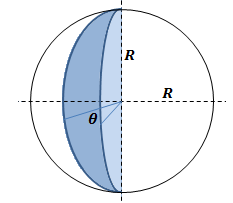
\includegraphics[width=1\textwidth]{wedge.png}
        \end{center}
      \end{column}
    \end{columns}

    \pause

    It can be shown that $\omega_d(S^{d-1}) = d\lambda_d(B^d)  = \frac{2 \pi^{d /
        2}}{\Gamma\left(\frac{d}{2}\right)} $.

    \begin{equation*}
      \sigma_{d}(A):= \omega_d(S^{d-1})^{-1} \omega_d(A)
    \end{equation*}

    is the \textbf{uniform probability distribution on the sphere}.

  \end{frame}

  \begin{frame}{Polar change of variables}
    \begin{theorem}
      \begin{itemize}
      \item $\sigma_{d}$ is the unique probability measure on the sphere
        $S^{d-1}$ invariant to the action of vectorial isometries.

        \pause

      \item For any measurable function $f: \Rd \to \R$ positive or integrable,

        \begin{equation*}
          \begin{aligned}
            \int_{\R^{d}} f(x) d x &=\int_{S^{d-1}}\left(\int_{0}^{\infty} f(r \gamma) r^{d-1} d r\right) d \textcolor{blue}{\omega_d}(\gamma) \\  &= \omega_d(S^{d-1})^{-1} \int_{S^{d-1}}\left(\int_{0}^{\infty} f(r \gamma) r^{d-1} d r\right) d \sigma_d(\gamma)
          \end{aligned}
        \end{equation*}


      \end{itemize}

    \end{theorem}

  \end{frame}

  \begin{frame}{Link to the Gaussian distribution}
    \begin{proposition}[Exercise 3.3.7] Let us write $X \sim N_d\left(0, I_{d}\right)$ in
      polar  form as
      $$
      X=R \theta
      $$
      where $R=\|X\|_{2}$ is the length and $\theta=X /\|X\|_{2}$ is the direction
      of $X$. Prove the following:

      \begin{enumerate}
      \item the length $R$ and direction $\theta$ are independent random variables
      \item the direction $\theta$ is uniformly distributed on the unit sphere
        $S^{d-1}$
      \item (Bonus) the length $R$ follows a generalized gamma distribution
      \end{enumerate}
    \end{proposition}

  \end{frame}

  \begin{frame}{Gaussian concentration}
  Recall theorem Isak, more hindsight from the exercise.
  \end{frame}
\end{document}
